\documentclass{article}
\usepackage[preprint]{neurips_2019}
\usepackage{graphicx,float}
% \usepackage[utf8]{inputenc} % allow utf-8 input
% \usepackage[T1]{fontenc}    % use 8-bit T1 fonts
% \usepackage{hyperref}       % hyperlinks
\usepackage{url}            % simple URL typesetting
% \usepackage{booktabs}       % professional-quality tables
% \usepackage{amsfonts}       % blackboard math symbols
% \usepackage{nicefrac}       % compact symbols for 1/2, etc.
% \usepackage{microtype}      % microtypography
\title{Predicting Stocks Trends Based on News}
\author{
Harsh Dedhiya, Raghav Malhotra, Phumin Walaipatchara\\
Department of Computer Science\\
Boston University\\
\texttt{hdedhiya@bu.edu, raghav20@bu.edu, phuminw@bu.edu}\\
}
\begin{document}
\maketitle
\begin{abstract}
The stock market is known to show emerging trends in the way of its computation and it is times
 of volatility that spontaneous judgments are needed to be made to speculate price behaviour.
 A platform which trains a predictive model through mining the news for headlines and words
 pertaining demonstrating an ascertainable correlation to share price changes is exemplary to
 the application of AI in finance. With the use of recurrent neural networks that incorporate LSTM,
 logistic regression, naïve bayes, term frequency and a simultaneous focus on political events keeping
 in mind the obsolete tendency. This attributes to the automation dynamic of the pertinent algorithms
 that would be amended to such occurrences.
 \\\\
 An example of this is, the dense implementation of blockchain in financial circulation that would
 give regulation less effective control of the financial industry and its cohorts. By this measure,
 the inability of the federal reserve to intervene in fabric of the stock market (with blockchain,
 monetary policy will not affect share prices). This is one conceptual aspect of several that call for
 existing models and algorithms to be subject to amendments. Cross validations are also performed between
 years and on a continuum to increase precision of the models and optimise them.
\end{abstract}
\section{Dataset}
Our first dataset was found at \url{https://www.kaggle.com/aaron7sun/stocknews}. This set included a file of the
 titles top 25 posts on reddit.com, from 2008-06-08 to 2016-07-01, with the date. Included as well is another
 dataset, which detailed statistics of the Dow Jones Industrial Average from Yahoo Finance, such as Open,
 Close, High, Low, Volume, and Adjusted Close for the same time span. Lastly, there was a combined dataset,
 which consolidated all 25 titles for a single day into 1 row, and added a Label column, which was determined
 as follows: 1 if the DJIA rose or stayed the same on the day, or 0 if it decreased. This was the dataset used
 for the Naive Bayes analysis, Logistic Regression analysis, and the Sentiment analysis. 
\\\\
Our second dataset was found at \url{https://www.kaggle.com/borismarjanovic/price-volume-data-for-all-us-stocks-etfs}.
 This set contained daily price and volume data for all US stocks and ETFs that were traded on the NYSE, NASDAQ,
 and NYSE MKT. Each company has its own csv file, and includes columns like Date, Open, High, Low, Close, Volume,
 OpenInt. Prices were adjusted for dividends and splits already. 
\\\\
Our third dataset was found at \url{https://www.kaggle.com/uciml/news-aggregator-dataset}. This dataset contained headlines
, URLs, Publisher, timestamp, and categories for 400,000+ news stories collected via a web scraper by UCI MLI. These news
 headlines are categorized into four classes, business, science and technology, entertainment, and health. These last two
 data sets were coordinated to use with the recurrent neural net.
\subsection{Preprocessing}
Because our first dataset set up the problem as a binary classification problem, but used very general headlines, getting
 the top 25 of a day, we decided to coordinate the two other datasets in a similar fashion, giving a label of whether the
 stock went up or down within a time period. We took advantage of the categories in the third dataset to get a labeled csv
 with only tech news, and made sure the titles included the company whose stock was used to label. Because not all news is
 released when the markets are open, we used the whichever open and close were the closest, starting with the same date,
 and iterating until we found a valid target. Labeling and filtering was done for 4 stocks,  AAPL, MSFT, GOOGL, and AMZN
 to be used with the RNN.
\section{Na\"ive Bayes}
This model was chosen because it was very simple, and could be used as a baseline. Again like the logistic regression,
 we performed this on the first dataset. We split the dataset by date, and used TF-IDF much like the last algorithm,
 but with 2-grams instead because of a lowered feature set. We again got chance level accuracy of .505 but found some
 interesting effectors. Positive effectors include “Al-Qaeda”, “Middle East”, “War Crimes”, and “Saudi Arabia”. Again
 like with logistic regression, we find a lexicon with words that contribute to war being positive effectors. Our negative
 effectors were also similar, including “phone hacking” and “nuclear weapons” much like before. However, the feature
 “wikileaks  founder” was a negative contributor in this model, while “wikileaks julian assange” was a postive contributor
 in the logistic regression. 
\\\\
Problems with this model are similar to the logistic regression, in that titles in the dataset were not necessarily relevant
 to the DJIA, and that the vocabulary used in the past is not necessarily the vocabulary used in the present.
\section{Logistic Regression}
This model was chosen because it is a standard when using categorical dependents, which binary classification presents.
 This was performed on the first dataset. First we split the dataset by date, with the training dataset being all the
 entries before 01/01/2015, and the testing dataset being the rest. We first fed the corpus of the training text into
 a TF-IDF vectorizer, removed stop-words, removed features that were too common, and features that were too rare, and
 then gave it to the model to predict the test data. We specified 3-gram features, so that we could identify patterns
 in the greatest effectors. Overall the accuracy of the model, given that it was a binary classification problem, was
 not more than chance, at .540. However, we found some interesting results in the effectors. Headlines with titles that
 included “nobel peace prize” and “human rights activist” were positive contributors, as well as titles like “soldiers
 killed afghanistan” and “gaza war crimes”. Historically, war has been a contributor to positive economic growth.
 The negative contributors were interesting as well,  with titles like “sentenced years jail”, “iran nuclear facilities”,
 and “phone hacking scandal” being among the most significant. These titles indicate that criminal activity often causes
 negative economic effects, which has also been observed.
\\\\
Some downfalls of this model were that the dataset included titles, regardless of whether they were relevant or not, which
 could lead to false positive correlations. Additionally, by parting the dataset by time, we failed to account for the fact
 that word usage and vocabulary changes over time. Thus training a model with word usage from a certain time period would
 lead to suboptimal results when testing the model on a different time period. The data should have been fetched more
 randomly from across the dataset.
\section{Sentiment Analysis}
For this method we again used the first dataset, but instead of using a TF-IDF to determine the feature space, we decided
 to feed the top 20 titles of the day to a sentiment analyzer called VADER. This is provided by NLTK, and is not a machine
 learning technique, but an algorithm that determines positivity, neutrality, negativity, and a compound score of a text
 based on features like capitalization, punctuation, proximity to qualifying adjectives and adverbs, and a lexicon of
 positive and negative words. We could have trained a model to do this ourselves, but we did not have labeled sentiments
 for each title, which would have made it easier. So we used the compound scores of each day to determine a mean
 sentiment for a day, and used that to train a logistic regression model. The thought behind this is that while the specific
 vocabulary of the titles might change over time, perhaps the general sentiment will still have the same effect on the DJIA.
 In this sense we used VADER to reduce the dimensionality of the text headlines to obtain a score for each day, and used the
 same labels as before to train. Again this resulted in a chance level accuracy of .489.
\\\\
This again suffered from the same problem of the headlines not being specific enough, which led us to finding our second
 and third datasets, which allowed us to filter by category, and gave us enough data such that we could ensure titles had
 the stock in the name.
\section{Recurrent Neural Network}
\indent In order to capture the objective of accurate prediction, Recurrent Neural Network (RNN) is introduced
 because its ability to exhibit internal state (memory). Specifically, Long short-term memory (LSTM),
 a special kind of RNN, is used for implementation as LSTM can deal with vanishing gradient problems
 and is capable of learning long-term dependencies.
\\
\begin{figure}
    \centering
    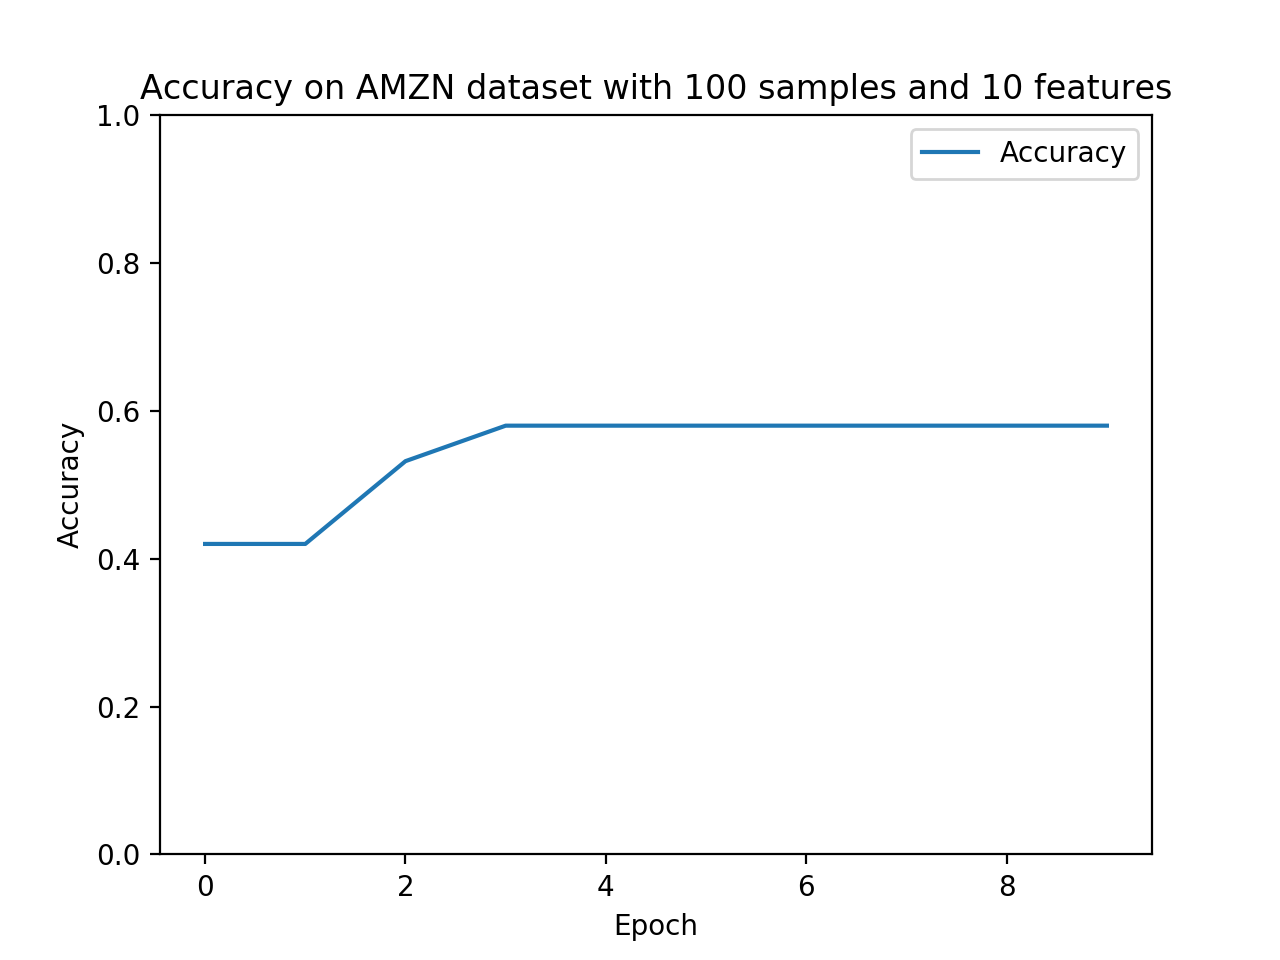
\includegraphics[scale=0.4]{assets/Accuracy.png}\\
    \caption{Accuracy of the model}
\end{figure}
\begin{figure}
    \centering
    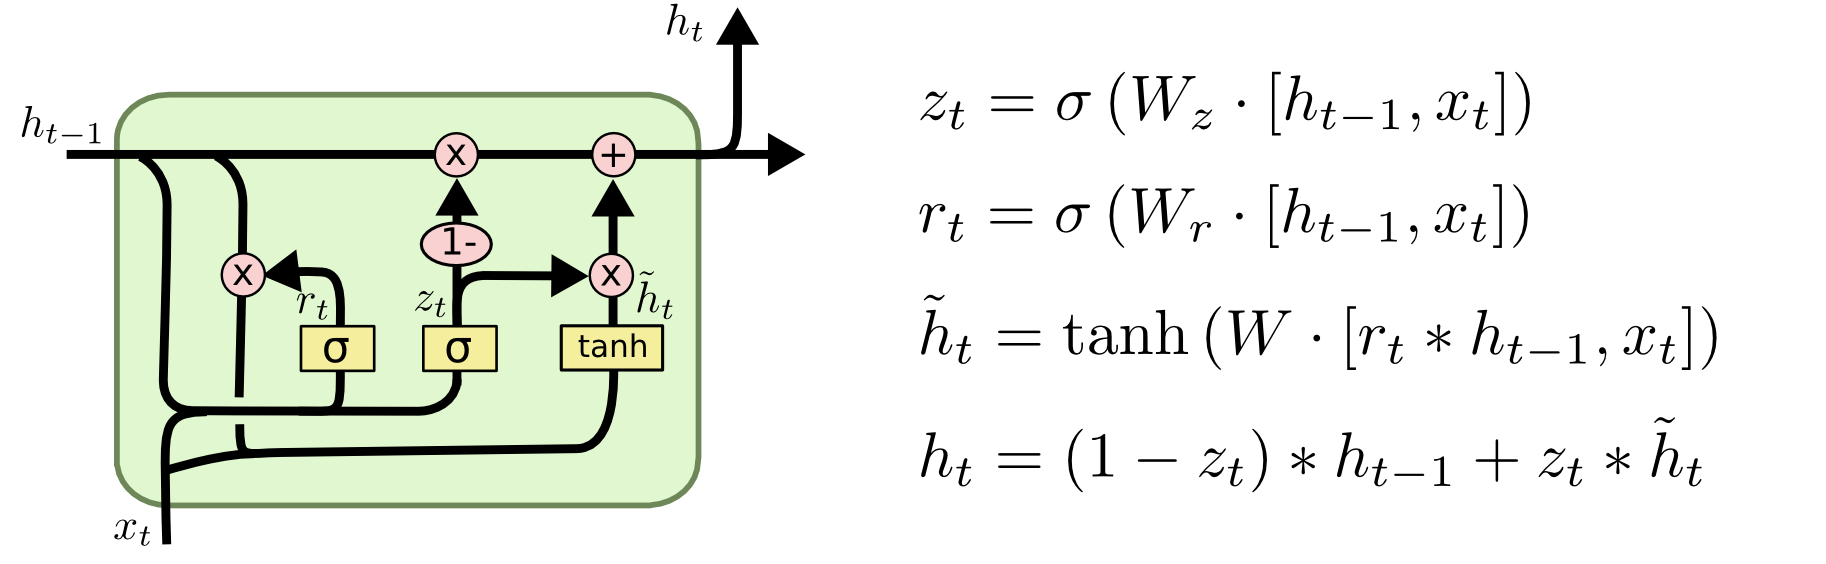
\includegraphics[scale=0.4]{assets/LSTM.png}
    \caption{LSTM structure}
\end{figure}
Before begin training the model, the dataset, 100 samples in this case, must be preprocesed introduced
 boolean vector through $TfidfVectorizer$ from $sklearn.feature\_extraction.text$. The $max_features$, which is
 also the size of the boolean vector is specified to be 10. Each sample (now a boolean vector) is paired up with
 the stock (AMZN in this case) movement, 1 for going up and 0 otherwise. In one epoch, we use $KFold$ from
 $sklearn.model\_selection$ to split the dataset into 2 groups, one for training and one for testing.
\\\\
 Regarding network structure, the LSTM network has 10 input nodes, which corresponds to the size of
 the boolean vector. It has 4 hidden nodes between the input layer and the LSTM and use sigmoid as an activation
 function. After LSTM module, the output layer consisting of 2 nodes uses softmax as an activation function in order
 to represent output as a probability of classification.
\\\\
During the training period of the network, the parameters (learning rate, $max\_feature$, and number of sample) have
 to be adjusted to some specific configuration in order to show the improvement of training as shown in Figure 1.
 Greater or lesser the value of parameters will result in stationary accuracy since the first epoch, which is not
 useful for parameter tuning process and training process.
\\\\
Currently, the only indicator that was taken into account is news headlines as a boolean vector through $TfidfVectorizer$.
 However, there are more factors that can be used as indicators for prediction, for instance, the unemployment rate,
 volume, social network, interest rate, etc. Those indicators should be fed into the network as well, but they need
 to be processed/weighted appropiately proportional to the importance of each indicator. As described, there are lots
 of rooms for improvement for this network and also for integrating other techniques to improve the accuracy of prediction.
\end{document}
